%\documentclass[a4paper]{article}
\documentclass{llncs}

\usepackage[T1]{fontenc}
\usepackage[utf8]{inputenc}

\usepackage{multirow}

\usepackage{graphicx}
\usepackage{xstring}
\usepackage{xspace}
\usepackage{amstext}

%\usepackage{showframe}
\usepackage{times}

\newcommand{\UNSAFE}{{\color{red!50!black} UNSAFE}\xspace}
\newcommand{\SAFE}{{\color{green!50!black} SAFE}\xspace}
\newcommand{\NA}{{\color{blue!50!black} N/A}\xspace}
\newcommand{\TODO}{{\color{red}\bf TODO}\xspace}
\newcommand{\DiH}{Diffie-Hellman\xspace}
\newcommand{\proverif}{ProVerif\xspace}
\newcommand{\ofmc}{OFMC\xspace}
\newcommand{\spear}{SPEAR II\xspace}
\newcommand{\opcua}{OPC-UA\xspace}
\newcommand{\opc}{OPC\xspace}
\newcommand{\dcom}{DCOM\xspace}
\newcommand{\mms}{MMS\xspace}
\newcommand{\iec}[1]{IEC\xspace#1\xspace}
\newcommand{\iccp}{ICCP\xspace}
\newcommand{\modbus}{MODBUS\xspace}
\newcommand{\profinet}{PROFINET\xspace}
\newcommand{\etherip}{EtherNet/IP\xspace}
\newcommand{\dnp}{DNP3\xspace}
\newcommand{\eg}{{\em e.g.}\xspace}
\newcommand{\etal}{{\em et al.}\xspace}
\newcommand{\securechan}{{\em OpenSecureChannel}\xspace}
\newcommand{\session}{{\em CreateSession}\xspace}

\title{Short paper: Domain Specific Filtering With Worst-Case Bandwidth}
\author{Maxime Puys \and Jean-Louis Roch \and Marie-Laure Potet}
\institute{Verimag, University Grenoble Alpes,  Gi\`eres, France \\
  \texttt{firstname.lastname@imag.fr}
  \thanks{This work has been partially supported by the LabEx PERSYVAL-Lab
      (ANR-11-LABX-0025) and the project {\em Programme Investissement d’Avenir
      FSN AAP Sécurité Numérique n\textsuperscript{o}3} ARAMIS (P3342-146798).}
}
\date{}

\begin{document}

\maketitle

\begin{abstract}
    Industrial systems are publicly the target of cyberattacks since
    Stuxnet \cite{Lan11}.  Nowadays they are increasingly communicating over
    insecure media such as Internet.  Due to their interaction with
    the real world, it is crucial to ensure their security. In this paper, we
    propose a stateful type of domain specific filtering able to keep track
    of the value of predertemined variables. Such filter allows to express rules
    depending on the context of the system. Moreover, it must guarantee bounded
    memory and execution time to be resilient against malicious adversaries.
    Our approach is illusrated on an example.
\end{abstract}

\section{Introduction}\label{sec:intro}
Industrial systems also called SCADA (Supervisory Control And Data
Acquisition) have been known to be targeted by cyberattacks since the
famous Stuxnet case~\cite{Lan11} in 2010.  Due to the criticity of
their interaction with the physical world, these systems can
potentially be really harmful for humans and environment.  The
frequence of such attacks is increasing to become one of the priorities for
governmental agencies (\eg~\cite{SFS11} from the US National Institute of
Standards and Technology (NIST) or
\cite{ANSSI12_guide_securite_industrielle_en} from the French {\em Agence
nationale de la sécurité des systèmes d'information} (ANSSI)).
%As
%industrial systems historically have been physically isolated from the
%rest of the world, there were less exposed to cyber attacks and their
%security was less considered. Nowadays, such attacks become feasible
%because these systems are spreading geographically and communicating
%more and more through unsafe mediums like Internet.


%Industrial systems have specificities. First the isolation of such
%systems requires the attacker to be physically present in the
%system. Then compagnies focused more on the protection against natural
%deceases and human mistakes than cybersecurity (often call security).
%In the context of security there is an adversary willing to perform malicious
%actions.
Industrial systems differ from other systems because of
the really long lifetime of there devices and their difficulty to
patch in case of vulnerabilities.
Such specificities encourage to carefully check
standards and applications before deploying them.
%It also explain the number of legacy hosts.
%Moreover, most of industrial protocols are proprietary and
%provide a very low level of security if
%any, \eg \modbus~\cite{MODBUS}, \profinet~\cite{PROFINET}, \etherip~\cite{Bro01}
%or
%\dnp~\cite{CR04}.
%However, in 2006, the {\em OPC Foundation} (an industry consortium)
%released the first version of \opcua~\cite{MLD09}, which is presented
%as the new standard for industrial communications. %% This standard  and whose security
%% is quite closer to business IT's protocols such as TLS~\cite{DR08}.
%% This directly applies to communication protocols.
As it already appeared for business IT's protocols for twenty years,
automated verification is crucial in order to discover flaws in the
protocols' specifications before assessing implementations. However,
the lack of formal verification of industrial protocols has been
emphasized in 2006 by Igure et al.~\cite{ILW06} and in 2009 by
Patel \emph{et al.}~\cite{PBG09}.  They particularly argued that
automated protocol verification allows to understand most of the
vulnerabilities of a protocol before changing its standards which
helps at minimizing the number of revisions which costs time and
money.  Moreover, due to the combinational explosion of the number of
possible execution traces and the increasing complexity of the
systems, only automated verification can ensure the security of a
protocol in a given model.

\TODO Intruduire \opcua qq part


%\subsection{State-of-the-art}\label{sec:intro_sota}
\paragraph{State-of-the-art:}\label{sec:intro_sota}

%The security of industrial protocols becomes a hot topic and some works are
%present in the literature.
Most of the works on the security of industrial protocols only rely on
specifications written in human language rather than using formal methods.
In 2004, Dzung et al. proposed a detailed survey on the security in SCADA
systems including analysis on the security properties offered by \opc (Open
Platform Communications), \mms (Manufacturing Message Specification),
\iec{61850}, \iccp (Inter-Control Center Communications Protocol) and \etherip.
Still in 2004, Clarke et al.~\cite{CR04} discussed the security of \dnp
(Distributed Network Protocol) and \iccp.
In 2006, in the technical documentation of \opcua (OPC Unified Architecture) the
authors detailled the security measures of the protocol (specialy in part 2, 4
and 6).
In 2015, Wanying et al. summarizeed the security offered by \modbus, \dnp and
\opcua.

On the other hand, some works propose new versions of existing protocols to make
them secure against malicious adversaries.
In 2007, Patel et al.~\cite{PY07} studied the security of \dnp and proposed two
ways of enhancing it through digital signatures and challenge-response models.
In 2009, Fovino et al.~\cite{FCMT09} proposed a secure version of \modbus
relying on well-known cryptographic primitives such as RSA or SHA2.
%This version of the protocol also need to introduce new components in the system
%to allow existing devices to use these cryptographic primitives.
In 2013, Hayes et al.~\cite{HE13} designed another secure \modbus protocol using
hash-based message authentication codes (HMACs) and built on STCP (Stream
Transmission Control Protocol).

To the best of our knowledge, the only work directly making use of formal
methods to prove the security of industrial protocols or find attack against
them is from Graham et al.~\cite{GP05} in 2005.
They proposed a formal verification of \dnp using \ofmc~\cite{BMV03} and
\spear~\cite{SH01}.
%% \TODO Sadly we were not able to access their modelings to discuss them with
%% ours.
%In 2008, Dutertre~\cite{Dut08} detailed formal specifications of \modbus
%developed using PVS, a generic theorem prover in order to help proving the
%consistancy of an implementation with the standards.

%\subsection{Contributions}
\paragraph{Contributions:}

We propose a formal analysis of the security of
% standard \modbus protocol and
%the correction proposed in~\cite{FCMT09}.%,HE13}.
%We also assess the 
the sub-protocols involved in the \opcua handshake, namely \opcua
OpenSecureChannel and \opcua CreateSession.  We are able to find
attacks against both of them and provide some countermeasures when
needed.  This work makes use of one of the most efficient tools in the
domain of cryptographic protocol verification according
to \cite{LP15}, namely \proverif developed by Blanchet et al.~\cite{Bla01}.
It analyzes a protocol written either in Horn clauses format or using
a subset of the Pi-calculus for an unbounded number of sessions
considering the classical Dolev-Yao intruder model~\cite{DY81}.  This
powerful intruder controls the network, listens, stops, forges,
replays or modifies some messages according to its capabilities and
knowledge.  The perfect encryption hypothesis is assumed, meaning that
it is not possible to decrypt a ciphertext without its encryption key
or to forge a signature without knowing the secret key.  In this
context, verification tools are able to verify security properties of
a protocol such as secrecy and authentication.  The first property
ensures that a secret message cannot be discovered by an unauthorized
agent (including the intruder).  The authentication property means
that one participant of the protocol is guaranteed to communicate with
another one.

\paragraph{Outline:} In the Section~\ref{sec:secure_channel}, we analyse the
security of \opcua OpenSecureChannel and 
\opcua CreateSession in Section~\ref{sec:session}. Finally, we conclude in Section~\ref{sec:conclusion}.


\section{Stateful Filtering}\label{sec:stateful}
\subsection{Description}\label{sec:stateful_desc}
Stateful = garder en mémoire la valeur de certaines variables.
Limites:
\begin{itemize}
    \item Mémoire et temps d'exécusion borné (cas des automates à piles ou du tri).
    \item Décision locale implique logique ternaire.
\end{itemize}

Modèles de l'adversaire.


\subsection{Proposed Implementation}\label{sec:stateful_impl}
\input{stateful_impl}

\section{Use-Case Example: an Electrical Disconector}\label{sec:example}
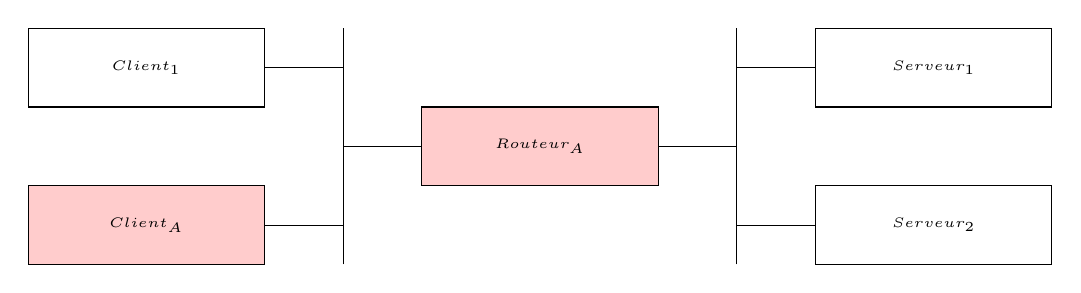
\begin{tikzpicture}[font=\tiny,
    arrow/.style={thick,<->,shorten >=2pt,shorten <=2pt,>=stealth},
]
    \draw[fill=red!20!white] (0,0) rectangle (3,1) node [pos=.5] {$Client_{A}$};
    \draw (0,2) rectangle (3,3) node [pos=.5] {$Client_1$};
    
    \draw[fill=red!20!white] (5,1) rectangle (8,2) node [pos=.5] {$Routeur_{A}$};

    \draw (10,0) rectangle (13,1) node [pos=.5] {$Serveur_{2}$};
    \draw (10,2) rectangle (13,3) node [pos=.5] {$Serveur_{1}$};
    
    \draw (3,.5) -- (4,.5); 
    \draw (3,2.5) -- (4,2.5); 
    \draw (4,1.5) -- (5,1.5);
    \draw (4,0) -- (4,3);

    \draw (9,.5) -- (10,.5); 
    \draw (9,2.5) -- (10,2.5); 
    \draw (8,1.5) -- (9,1.5);
    \draw (9,0) -- (9,3);
\end{tikzpicture}


\section{Conclusion}\label{sec:concl}
In this paper we present a stateful type of domain specific filtering able to
keep track of the value of predetermined variables.
It guarantees bounded memory and execution time to be resilient against
malicious adversaries since processing one command only depends on the number of
rules and memory to store monitor is controlled by only monitoring scalar
variables (or cells when multidimensional).

In the future, we plan on extending the boolean predicates to handle more
complex arithmetic such has "$Equal(2*NewVal+1, LocalVal[1]^2)$".
Such verification are still performed in constant time since we are only
evaluating the expression with concrete values.
We would also be able to specify rules to avoid {\em Denial-of-service}.
Such rules would limit the number of access to a certain variable within a
period of time (\eg no more than 10 Read commands per minute) while keeping
our bounded time and memory properties.


\bibliographystyle{unsrt}
\bibliography{phdBiblio}

\end{document}
